
\begin{figure}
\centering

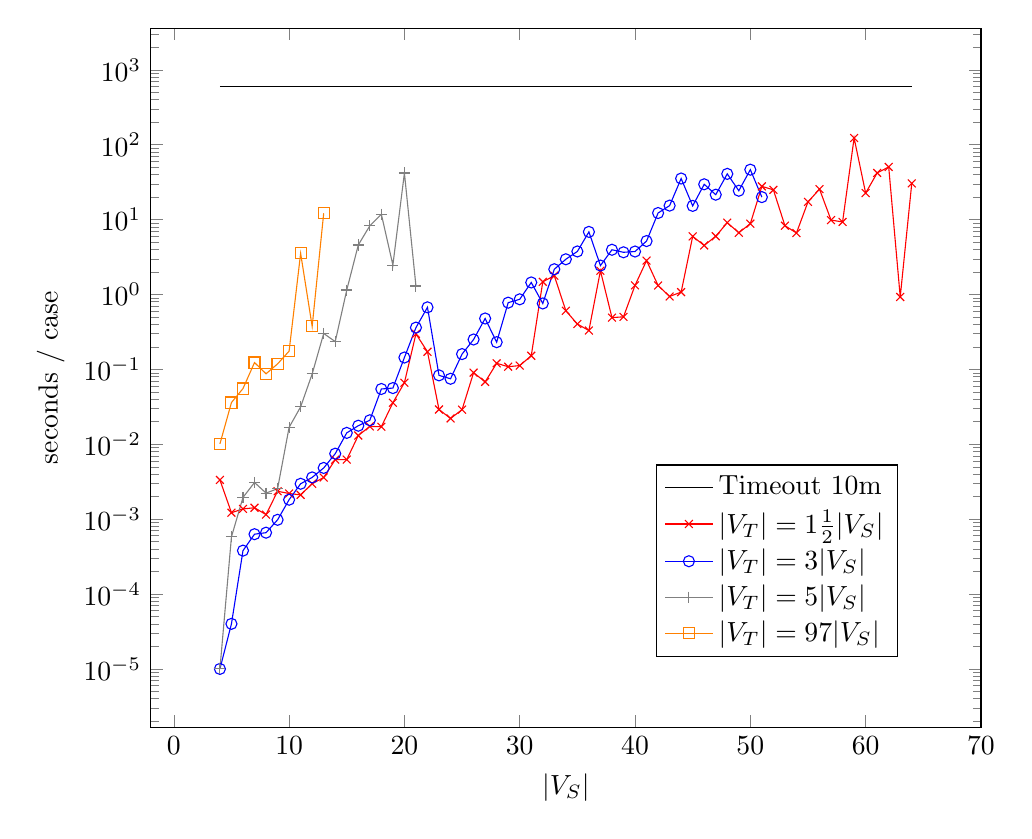
\begin{tikzpicture}
    \begin{axis}[
        xlabel=$|V_S|$,
        ylabel=seconds / case,
        ymode=log,
        legend style={at={(0.9,0.1)},anchor=south east},
        width=\textwidth,
        legend cell align={left},
		%y tick label style={/pgf/number format/sci},
    ]
    
    \addplot[
        mark=none,
        black,
    ] plot coordinates {
        (4,600)
        (64,600)
};
    \addlegendentry{Timeout 10m} 

	\addplot[
        mark=x,
        red,
    ] plot coordinates {
        (4,0.0033400000000000014)
        (5,0.001220000000000001)
        (6,0.001370000000000001)
        (7,0.001420000000000001)
        (8,0.0011500000000000008)
        (9,0.002360000000000002)
        (10,0.0022000000000000014)
        (11,0.0021100000000000016)
        (12,0.0029700000000000017)
        (13,0.003600000000000002)
        (14,0.006230000000000005)
        (15,0.006250000000000005)
        (16,0.013089999999999997)
        (17,0.01733999999999998)
        (18,0.017149999999999988)
        (19,0.035899999999999974)
        (20,0.06641000000000002)
        (21,0.29804999999999987)
        (22,0.17200000000000004)
        (23,0.029129999999999993)
        (24,0.022129999999999986)
        (25,0.02902999999999998)
        (26,0.09048999999999996)
        (27,0.06807999999999997)
        (28,0.12055999999999999)
        (29,0.10859999999999997)
        (30,0.11245999999999994)
        (31,0.15224000000000001)
        (32,1.4779599999999993)
        (33,1.7825299999999984)
        (34,0.6063999999999998)
        (35,0.40355)
        (36,0.330344827586207)
        (37,2.0783100000000005)
        (38,0.49150000000000005)
        (39,0.5033899999999999)
        (40,1.32485)
        (41,2.8371999999999997)
        (42,1.3199200000000002)
        (43,0.9420099999999999)
        (44,1.0761999999999998)
        (45,5.976269999999999)
        (46,4.51925)
        (47,5.99943)
        (48,9.102549295774647)
        (49,6.678814814814815)
        (50,8.834840579710145)
        (51,27.791812499999995)
        (52,24.997499999999988)
        (53,8.305178082191782)
        (54,6.6299382716049395)
        (55,17.260810810810817)
        (56,25.533208333333338)
        (57,9.857642857142858)
        (58,9.315249999999999)
        (59,122.99537500000002)
        (60,22.631678571428576)
        (61,42.039571428571435)
        (62,50.52257142857143)
        (63,0.9269999999999999)
        (64,30.450666666666663)
};
    \addlegendentry{$|V_T|=1\frac{1}{2}|V_S|$}
    
    
    \addplot[
        mark=o,
        blue,
    ] plot coordinates {
        (4,1.0E-5)
        (5,4.0E-5)
        (6,3.800000000000003E-4)
        (7,6.300000000000005E-4)
        (8,6.600000000000004E-4)
        (9,9.800000000000008E-4)
        (10,0.0018200000000000013)
        (11,0.0029700000000000017)
        (12,0.003610000000000002)
        (13,0.0048300000000000036)
        (14,0.0074900000000000045)
        (15,0.014199999999999996)
        (16,0.017699999999999994)
        (17,0.020929999999999987)
        (18,0.05475999999999996)
        (19,0.05629999999999999)
        (20,0.14404999999999996)
        (21,0.36141000000000006)
        (22,0.6743300000000008)
        (23,0.08323999999999998)
        (24,0.07494999999999995)
        (25,0.16018999999999994)
        (26,0.25077999999999995)
        (27,0.4785799999999999)
        (28,0.23094999999999996)
        (29,0.7784899999999998)
        (30,0.8627700000000003)
        (31,1.4490600000000011)
        (32,0.75956)
        (33,2.1747600000000005)
        (34,2.955129999999999)
        (35,3.758652173913044)
        (36,6.86023913043478)
        (37,2.4347647058823525)
        (38,3.958900000000001)
        (39,3.662639999999999)
        (40,3.75055)
        (41,5.173680000000003)
        (42,12.2565306122449)
        (43,15.383380952380952)
        (44,35.409058823529406)
        (45,15.255863636363637)
        (46,29.63761904761904)
        (47,21.52631428571429)
        (48,40.831)
        (49,24.304000000000006)
        (50,46.49093333333334)
        (51,19.994428571428575)
};
    \addlegendentry{$|V_T|=3|V_S|$}
   
   
   \addplot[
        mark=+,
        gray,
    ] plot coordinates {
        (4,1.0E-5)
        (5,5.800000000000003E-4)
        (6,0.0019500000000000012)
        (7,0.0030900000000000016)
        (8,0.002230000000000001)
        (9,0.002550000000000001)
        (10,0.016829999999999987)
        (11,0.03163999999999996)
        (12,0.08694999999999997)
        (13,0.3020299999999999)
        (14,0.23475000000000004)
        (15,1.1472800000000003)
        (16,4.5852900000000005)
        (17,8.272409090909091)
        (18,11.811108695652175)
        (19,2.473866666666667)
        (20,41.929625)
        (21,1.2983333333333336)
        (22,NaN)
};
    \addlegendentry{$|V_T|=5|V_S|$}
    
    
    \addplot[
        mark=square,
        orange,
    ] plot coordinates {
        (4,0.010120000000000004)
        (5,0.03607999999999999)
        (6,0.05543902439024388)
        (7,0.12339024390243905)
        (8,0.08742)
        (9,0.11838999999999995)
        (10,0.17537209302325582)
        (11,3.546875)
        (12,0.3752857142857143)
        (13,12.16516666666667)
};
     \addlegendentry{$|V_T|=97|V_S|$}

    \end{axis}
    \end{tikzpicture}


\caption{Performance of our algorithm $\mathit{RTSH}$ using the configurations that individually perform best: DFS path iteration, avoiding unnecessarily long paths and N-reachability AllDifferent pruning. Contraction is disabled. We use 10 minutes worth of tests for each data point and stop testing when that is not enough for finding a homeomorphism in a single test case.}
\label{fig:highperformance}
\end{figure}
